\section{Appendix} \label{appendix B}
\textbf{Proof that $\displaystyle{\boldsymbol{\lim_{n \rightarrow \infty}\brac{1 + \frac{x}{n}}^n = e^x.}}$}\\

\noindent Consider the following graph of the real valued function $f(t) = \frac{1}{t}$,

\begin{center}
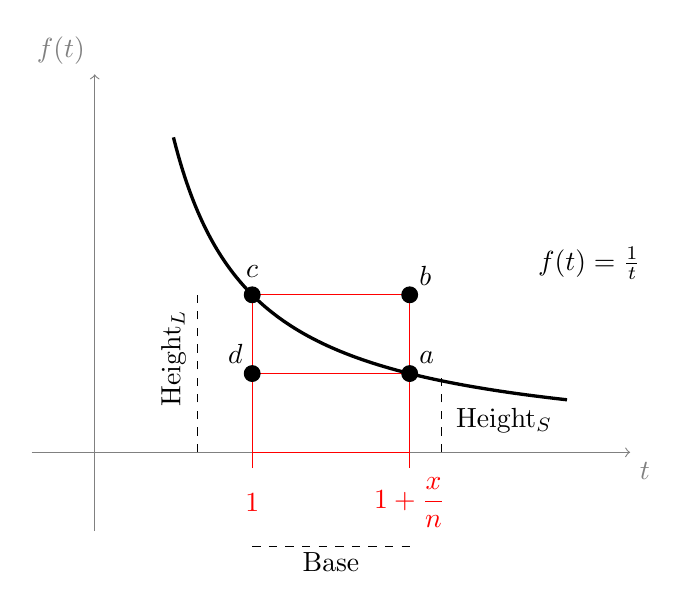
\begin{tikzpicture} [scale = 2]
\draw[very thick, domain=0.5:3, samples=200, smooth] plot (\x, {1/\x});
\draw [gray, ->] (0,-0.5) -- (0,2.4) node [above left] {$f(t)$};
\draw [gray, ->] (-0.4,0) -- (3 + 0.4,0) node [below right] {$t$};
%\foreach \s in {-0.5,-0.6,-0.7,-0.4,-0.3,-0.2,-0.1,0,0.1,0.2,0.3,0.4,0.5,0.6,0.7,0.8,0.9,1,1.1,1.2,1.3,1.4,1.5,1.6,1.7,1.8,1.9,2,2.1,2.2,2.3} {
%\draw [opacity = 0.3, gray] (-0.4,\s) -- (3.5 + 0.4, \s);
%}
\node [fill = white] at (pi,1.2) {$f(t) = \frac{1}{t}$};
%	\foreach \s in {0,1/9,2/9,3/9,4/9} {
%	\draw [red] (\s*4*pi,-0.1) -- (\s*4*pi,0.1);
%	}
\draw [red] (2,0.1) -- (2,1) -- (1,1);
\draw [red] (1,0) -- (2,0);
\draw [red] (1,1/2) -- (2,1/2);
\draw [red] (2,0.1) -- (2,-0.1) node [below] {$\displaystyle{1 + \frac{x}{n}}$};
%\draw [red] (2*pi,0.1) -- (2*pi,-0.1) node [below] {$2\pi$};
\draw [red] (1,-0.1) -- (1,1);
\node [red] at (1,-0.32) {$\displaystyle{1}$}; 
\draw [fill = black] (2,1/2) circle (0.05cm) node [above right] {$a$};
\draw [fill = black] (1,1/2)  circle (0.05cm) node [above left] {$d$};
\draw [fill = black] (1,1)  circle (0.05cm) node [above = 1mm] {$c$};
\draw [fill = black] (2,1)  circle (0.05cm) node [above right] {$b$};
\draw [dashed] (1,-0.6) -- (2,-0.6);
\node at (1.5,-0.7) {Base};
\draw [dashed] (0.65,0) -- (0.65,1);
\node [rotate = 90] at (0.5,0.6) {Height$_L$};
\draw [dashed] (2.2,0) -- (2.2,0.5); 
\node at (2.6,0.2) {Height$_S$};
%\draw [red] (0.1,1) -- (-0.1,1) node [left] {$\frac{320}{9}$};
%\draw [red] (0.1,-1) -- (-0.1,-1) node [left] {$-\frac{320}{9}$};
\end{tikzpicture}
\end{center}
The distance from $1$ to $1 + \frac{x}{n}$, along the $t$-axis, is labelled ``Base.'' This distance is given by
\[
\text{Base} = \brac{1 + \frac{x}{n}} - 1 = \frac{x}{n}.
\]
The distance along the line segment from $t = 1$ on the $t$-axis, to the point labelled $c$, is labelled Height$_L$. This distance is given by
\[
\text{Height$_L$} = f(1) = 1.
\] 
The distance along the line segment from $t = 1 + \frac{x}{n}$ on the $t$-axis, to the point labelled $a$ is labelled Height$_S$. This distance is given by,
\[
\text{Height$_S$} = f(1 + \frac{x}{n}) = \frac{1}{1+\frac{x}{n}}.
\]
We will label the large rectangle $R_{L}$; this is the rectangle bordering the $t$-axis and passing through the points $b$ and $c$. It has area
\[
\text{Area($R_L$)} = \text{Base}\times \text{Height$_L$} = \frac{x}{n} \times 1 = \frac{x}{n}
\]
We will label the small rectangle $R_{S}$; this is the rectangle bordering the $t$-axis and passing through the points $a$ and $d$. It has area
\[
\text{Area($R_S$)} = \text{Base}\times \text{Height$_S$} = \frac{x}{n} \times \frac{1}{1+\frac{x}{n}} = \frac{x}{n + \frac{nx}{n}} = \frac{x}{n + x}.
\]
We will use the label ``Area(Curve)'' to refer to the area under the curve $f(t)$, from $t = 1$ to $t =1 + \frac{x}{n}.$ This area is given by the integral
\[
\text{Area(Curve)} = \int_1^{1+\frac{x}{n}} f(t) \ud t = \int_1^{1+\frac{x}{n}} \frac{1}{t} \ud t.
\]
Notice from the diagram that
\[
\text{Area($R_S$)} \leq \text{Area(Curve)} \leq \text{Area($R_L$)}. \\
\]
Substituting in the expressions that we have found gives
\[
\frac{x}{n+x} \leq \int_1^{1+\frac{x}{n}} \frac{1}{t} \ud t \leq \frac{x}{n}.
\]
Evaluating the integral gives
\[
\frac{x}{n+x} \leq \ln \brac{1 + \frac{x}{n}} - \ln(1) \leq \frac{x}{n}.
\]
Multiplying the whole expression by $n$, and noting that $\ln(1) = 0$, we get
\[
\frac{nx}{n+x} \leq n\ln \brac{1 + \frac{x}{n}} \leq x.
\]
Using the logarithm power rule $\squac{a\ln(b) = \ln(b^a) \; \text{for all $b > 0$, and $a \in \R$}}$, we get 
\[
\frac{nx}{n+x} \leq \ln \brac{\brac{1 + \frac{x}{n}}^n} \leq x.
\]
Taking the Exponential function of the whole expression gives,
\[
\e^{\frac{nx}{n+x}} \leq e^{\ln \brac{\brac{1 + \frac{x}{n}}^n}} \leq \e^x
\]
Since Exponential is inverse to natural logarithm the middle term simplifies and we get
\[
e^{\frac{nx}{n+x}} \leq \brac{1 + \frac{x}{n}}^n \leq \e^x
\]
Now, as $n \rightarrow \infty$, the expression $\frac{n}{n+x}$ approaches 1, so $\frac{nx}{n+x}$ approaches $x$. Thus, as $n \rightarrow \infty$, the expression $e^\frac{nx}{n+x}$ approaches $e^x$. Hence, as $n$ approaches infinity we get
\[
e^x \leq \brac{1 + \frac{x}{n}}^n \leq \e^x.
\]
We have \textit{squeezed} the expression $\brac{1 + \frac{x}{n}}^n$ between two terms, both $\e^x$. Hence we conclude that
\[
\lim_{n \rightarrow \infty}\brac{1 + \frac{x}{n}}^n = \e^x.
\]
Note that two important theorems about limits were implicitly used in this proof, though these theorems were not covered in this course. One is called the \textit{Squeeze Principle}; this theorem was used in the final step. The other is called \textit{Limit of a Composite}; this theorem was used when we said that $e^\frac{nx}{n+x}$ approaches $e^x$ when $\frac{nx}{n+x}$ approaches $x$. In this subject we never really gave the proper definition of a limit, but all of the calculus that we learned relies on limits! If you want to know more about limits, and how we truly make sense of these ideas, the subject, ``mathematical analysis'' deals with the topic in detail. \\

\subsubsection{Compound interest, natural growth, and the number $\e$}
Even if you have never studied compound interest, and you find compound interest completely unstimulating, it is possible that you'll find the following facts quite fascinating. The formula
\[
y = P\brac{1 + \frac{r}{n}}^n
\]
is a common formula used to calculate compound interest over one year. In this formula, the variable, $y$, represents the amount of money in an account after one year. The variable $P$ represents the intitial investment (i.e., the ``principle''), $r$ represents the interest rate that is compounded after every term, and $n$ represents the total number of terms in one year. If we let $P = r = 1$, i.e., if we invest \$1, at a compounding interest rate of 100\% per term, for a period of 1 year, then we get
\[
y =  \brac{1 + \frac{1}{n}}^n
\]
 Now, if we let $n$ get infinitely small, that is, if the interest is compounded \textit{continuously}, we get
 \[
 y = \lim_{n \rightarrow \infty}\brac{1 + \frac{1}{n}}^n = \e^1 = \e.
 \]
 This may give some insight into why $\e$ is such an important number (and why it is referred to as the ``natural'' number); it is the base rate of growth shared by all continuously growing (or decaying) processes. Just as every number can be expressed as a multiple of the number $1$, every continuous growth or decay rate can be expressed as a scaled version of $\e$.\\
 
\noindent Using $\e$, and the Exponential function, we can model the growth of organisms, the growth of populations, radioactive decay, and many, many other natural processes.

 
 